% By zmienic jezyk na angielski/polski, dodaj opcje do klasy english lub polish
\documentclass[polish, 12pt]{aghthesis}
\usepackage{babel}
\usepackage[utf8]{inputenc}
\usepackage{url}
\usepackage{indentfirst}
\usepackage{amsmath}
\usepackage{comment}
\usepackage{amsmath}
\usepackage{graphicx}
\usepackage{caption}
\usepackage{subcaption}
\usepackage{listings}

\author{Dawid Romanowski, Wojciech Czarny}

\title{Implementacja metody SPH \\ na procesory graficzne}

\supervisor{dr hab.\ inż.\ Krzysztof Boryczko, prof.\ nadzw.\ AGH}

\date{2014}

% Szablon przystosowany jest do druku dwustronnego, 
\begin{document}
\raggedbottom
\maketitle{}

\tableofcontents
\clearpage

	\section{Opis metody SPH}

		\subsection{Wstęp}
			
			Metoda Smoothed Particle Hydrodynamics (SPH) początkowo miała służyć do symulacji zjawisk astrofizycznych takich jak powstawanie galaktyk czy gwiazd. Zaproponowana niezależnie w 1977 roku prez Ginolda i Monaghana oraz Lucy obecnie jest często wykorzystywana do symulacji zjawisk w mniejszej skali - w szczególności zachowań płynów. 

			Ideą tej metody jest wyróżnienie pewnego dyskretnego zbioru węzłów (zwanych dalej cząstkami) badanego przez nas płynu, nadanie im pewnych własności fizycznych a następnie interpolacja tych własności fizycznych w pewnej przestrzeni. Do interpolacji wykorzystywane są funkcje wygładzające, które zamieniają punktową reprezentację wartości fizycznych na reprezentację przestrzenną.

			SPH jest metodą Langrange'owską z czego wynika, że cząski mogą się poruszać w czasie. W naszym modelu ograniczyliśmy się do trzech rodzajów sił działających na cząstki. Siła grawitacyjna, siła spowodowana różnicą ciśnień oraz lepkość.

		\subsection{Równanie Naviera-Stokesa}

			Metoda SPH jest oparta na równaniu hydrodynamicznym Naviera-Stokesa

			\[{\rho}[\frac{\partial v}{\partial t} + v \cdot \nabla v ]= F - \nabla p + \mu \nabla^2 v \label{eq:navier-stokes} \tag{1}\]

			\[{\rho}(\nabla \cdot v)=0 \label{eq:continuity} \tag{2}\]

			dla cieczy nieściśliwych, gdzie: ${\rho}$ to gęstość cieczy, ${\mu}$ to współczynnik lepkości a F reprezentuje zewnętrzne siły działające na ciecz.
			
			Analiza równania (\ref{eq:navier-stokes}) pokazuję, że przyspieszenie jest zależne jedynie od sił zewnętrznych działających na cząstkę, ujemnego gradientu ciśnienia układu oraz lepkości cieczy. Jedyna siła zewnętrzna, która interesuje nas w naszej pracy to siła grawitacji. Możemy więc zapisać: \[F={\rho}g \label {eq:gravity_force} \tag{3} \] Czynnik $v {\cdot} {\nabla} v$ reprezentuje przyspieszenie konwekcyjne, które jest efektem niezależnego od czasu przyspieszenia cząstek w zależności od przestrzeni. $-{\nabla}$p oznacza, że ciecz będzie się poruszać z przestrzeni o większym ciśnieniu w kierunku mniejszego ciśnienia. Lepkość reprezentowana jest jako stała lepkości razy laplasjan pola prędkości, który można interpretować jako różnicę między prędkością w danym punkcie a średnią prękością w małej otaczającej go przestrzeni. Lepkościa rozprasza pęd czątek i sprawia, że układ dąży do stanu równowagi.
			
			Równanie (\ref{eq:continuity}) jest po prostu równaniem zachowania masy. W naszej pracy nie było ono istotne ze względu na cechy metody SPH, które gwarantują, że jest ono spełnione w każdej sytuacji.
			 
		\subsection{Funkcje wygładzające}
			
			Celem funkcji wygładzającej jest transformacja reprezentacji cząstki z punktowej masy na przestrzenną. Funkcje wygładzające najczęściej przyjmują kształt zbliżony do rozkładu normalnego, należą conajmniej do klasy ${C^2}$ (mają ciągłą pierwsza i drugą pochodną) i są znormalizowane (całkują się do 1 od $-{\infty}$ do $+{\infty}$). Prostym przykładem takiej funkcji może być funkcja Gaussa \[W_G(r,h)=\frac{1}{h^{\nu}\pi^{{\nu}/2}}exp(-\frac{r^2}{h^2}) \label{eq:gaussian} \tag{4}\] gdzie ${\nu}$ to ilość wymiarów, r to odległość od od cząstki której estymujemy wielkość fizyczną i h to tak zwany promień wygładzania.
			
			Mając tak zdefiniowany promień wygładzania oraz dowolną dyskretną dystrybucję czątek, możemy estymować wartość fizyczną A w dowolnym punkcie przestrzeni i jako: \[{A}_i=\sum_{j=1}^{N}m_j\frac{A_j}{\rho_j}W(r_{ij},h_j) \label{eq:calc_all} \tag{5}\] gdzie ${r_{ij}}$ to odległość od cząstki j do punktu w przestrzeni, który rozważamy (pozycja i), ${m_j}$ to masa cząstki j, ${h_j}$ to promień wygładzania cząstki j, a suma jest po wszystkich cząstkach ze zbioru. 
			
			
			Przy doborze odpowiedniej funkcji wygładzającej W kluczową rolę odgrywa promień wygładzania h. Funkcja Gaussa nie jest używana do obliczeń ponieważ fakt, iż dąży ona do 0 w nieskończoności - rozciąga się w nieskończoność. Korzystając z niej, wszystkie cząstki brałyby udział przy obliczeniach w każdym punkcie. Jest to niepotrzebne, szczególnie kiedy cząstka jest bardzo odległa od rozpatrywanego punktu. Dlatego przeważanie dobiera się takie funkcje wygładzające, że dla ${r_{ij} > h}$ wartość funkcji wynosi 0. Przykładem takiej funkcji może być
			
			\[ W_{ij} = \frac{1}{\pi h^3} \left\{ 
				\begin{array}{l l l}
					1 - \frac{3}{2}(\frac{|r_{ij}|}{h})^2 + \frac{3}{4}(\frac{|r_{ij}|}{h})^3  & \quad \text{gdy ${0 \leq \frac{|r_{ij}|}{h} < 1}$}  \\ 
					\frac{1}{4}[2 - (\frac{|r_{ij}|}{h})]^3  & \quad \text{gdy ${1 \leq \frac{|r_{ij}|}{h} < 2}$}  \\ 
					0 & \quad \text{gdy ${\frac{|r_{ij}|}{h} \geq 2 }$} 
				\end{array} \right.\ \label{eq:kernel_function} \tag{6}\]
			\ \\
			zaproponowana przez Monaghana i Lattanzio w \cite{MonLat} czy:
			
			\[ W_{ij} = \left\{
				\begin{array}{l l}
					\frac{105}{16 \pi h^5}(1 + 3 \frac{|r_{ij}|}{h})(1-\frac{|r_{ij}|}{h})^3 & \quad \text{gdy ${|r_{ij}| \leq h}$}  \\ 0 & \quad \text{gdy ${|r_{ij}| > h}$} 
				\end{array} \right.\ \label{eq:kernel_function} \tag{7}\]
			\ \\
			opisywana w pozycji \cite{Lucy}
			
			My zdecydowaliśmy się wykorzystać drugą opcję, głównie ze względu na łątwiejszą implementację. 
			
			Kolejnym problemem przy doborze odpowiedniego promienia wygładzania jest to, zbyt duża lub zbyt mała wielkość może całkowicie zaburzyć wyniki eksperymentu.
			\begin{figure}[h!]
			\centering
			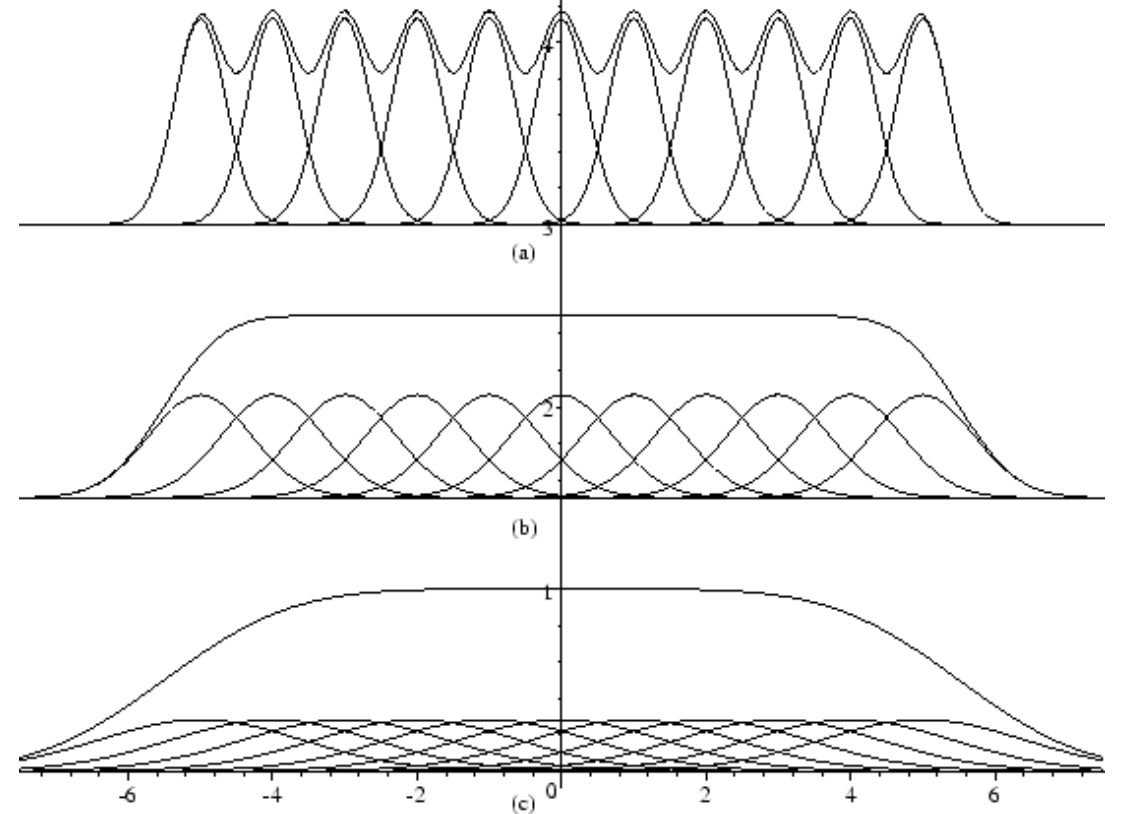
\includegraphics[width=0.8\textwidth]{smoothing.png}
			\caption{a) h=0.5 b) h=1 c) h=2}
			\label{fig:smoothing}
			\end{figure}
			Rysunek \ref{fig:smoothing} pokazuje co może się stać jeśli źle dobierzemy wartość promienia wygładzania. Pokazuje on równoodległe cząstki o tej samej wadze. Obliczona gęstość docelowo powinna przypominać linię ${\rho}$ = 1. Widać natomiast, że w c, gdzie dobraliśmy zbyt duże h linia ta znacząco przewyższa wartość oczekiwaną. Poprawnie dobrane h, do którego winniśmy dążyć, leży gdzieś pomiędzy przykładem a i b.
			
		\subsection{Wzory użytkowe}
			\subsubsection{Gęstość}
			Z równania (\ref{eq:calc_all}) gęstość w dowolnym punkcie możemy obliczyć korzystając ze wzoru \[{\rho}_i=\sum_{j=1}^{N}m_jW(r_{ij},h_j) \label{eq:calc_density} \tag{8}\] 
			\subsubsection{Równanie stanu}
			Jako równanie stanu wykorzystaliśmy zaproponowaną przez Monaghana w [Monaghan J.J. Sph without a tensile instability. J. Comp. Phys., 159:290-311, 1999.] funkcję:
			\[p_i(\rho)=\frac{\rho_0 c_0^2}{\gamma}[(\frac{\rho_i}{\rho_0})^{\gamma} - 1] \label{eq:calc_state} \tag{8}\]
			gdzie ${c_0}$ to prędkość dźwięku przy zadanej gęstości ${\rho_0}$, a ${\gamma}$ ma wartość 7, dzięki czemu płyn jest odporny na ściskanie. $\rho_0$ jest gęstością spoczynkową układu, do której dążyć będą wszystkie obszary gęstości. Łatwo zauważyć iż dzięki podniesieniu ilorazu gęstości do wysokiej potęgi (wskazana wartość wyznaczona została jako optymalna) nawet małe odchylenia gęstości powodować będą duże różnice ciśnienia, co uodparnia układ na ściskanie.
			
			Możliwe jest także użycie prostszego wyrażenia:	
			\[p_i(\rho) = k(\rho_0 - \rho_i) \tag{9}\]
			
			daje ono możliwość symulowania zachowań gazu, ponieważ umożliwia ściskanie w dużo większym stopniu niż ($\ref{eq:calc_state}$).
			
			\subsubsection{Różnica ciśnień}
			Przekształcenia opisane w \cite{Boryczko} pokazują, że skłądową sił pochodząca od ciśnienia, działającą na cząstkę i można zapisać jako: \[\frac{\nabla P_i}{\rho_i} = \sum_j m_j(\frac{P_j}{{\rho_j}^2} + \frac{P_i}{{\rho_i}^2})\nabla W(r_{ij}, h_j) \label{eq:calc_pressure} \tag{9}\] Gdzie ${\nabla}$W to piersza pochoda funkcji wygładzającej po odległości.
			
			\subsubsection{Lepkość}
			Oprócz oczywistego wzoru na lepkość wynikającego bezpośrednio z (\ref{eq:navier-stokes}) istnieje wiele innych modeli lepkości \cite{Boryczko}.
						
			W naszym projekcie wykorzystaliśmy model Monaghana ponieważ dawał zadowalające wyniki i był najmniej złożony obliczeniowo. Składnik ten wyrażony jest wzorem:
			
			\[{\Pi}_{ij} = \frac{-\alpha \mu_{ij} c_{ij} + \beta\mu_{ij}^2}{\rho_{ij}} \label{eq:viscosity_term} \tag{10}\]
	
			gdzie $\alpha$ i $\beta$ są parametrami modelu, a ich wartość zależy od oczekiwanych właściwości symulowanego płynu, $c_{ij} = (c_i + c_j) / 2$ (gdzie $c_i = (\gamma p_i / \rho_i)^\frac{1}{2}$ to prędkość dźwięku w miejscu $r_i$) oraz:
			
			\[{\mu}_{ij} = \left\{
				\begin{array}{l l}
					\frac{(v_i - v_j)\cdot(r_i - r_j)}{h_{ij}(||r_i - r_j||^2 / h_{ij}^2 + \eta^2)} & \quad if{(v_i - v_j)\cdot(r_i - r_j) < 0}  \\ 0 & \quad if{(v_i - v_j)\cdot(r_i - r_j) \geq 0} 
				\end{array} \right.\ \label{eq:mu_factor} \tag{11}\]
				
			Promień wygładzania obliczyć można jako $h_{ij} = (h_i + h_j)/2$, jednakże w naszym przypadku jest on zawsze stały, więc $h_{ij}$ zamienić można na $h$. Ta postać modelu lepkości jest kombinacją tzw. lepkości bulk (liniowa względem $\mu_{ij}$) oraz lepkości von Neumanna-Richtmeyera (kwadratowo zależna od $\mu_{ij}$). Lepkość von Neumanna-Richtmeyera zaproponowana została do symulacji uderzeń w celu zapobiegnięcia zjawisku przenikania się cząstek. 
			

			Jak wykazano w \cite{Lombardi}, wyniki najbliższe rzeczywistości można uzyskać przyjmując $\alpha \approx 0.5, \beta \approx 1.0$ oraz $\eta \approx 0.1$
	
	\section{GPGPU i OpenCL}
		
		\subsection{GPGPU}
			GPGPU (ang. General-Purpouse computing on Graphics Processor Units) to technika cechująca się wykorzystaniem GPU, które przeważnie zajmują się obliczeniami związanymi z grafiką komputerową, do dowolnych innych obliczeń. Technika ta znajduje zastosowanie głównie w obliczeniach równoległych ze względu na wykorzystanie w nowoczesnych kartach graficznych architektury SIMD (Single Instruction Multiple Data) i modelu wykonywania SIMT (Single Instruction Multiple Threads). GPU są obecnie zdolne wykonywać nawet tysiące wątków jednocześnie co sprawia, że znacząco lepiej radzą sobie z algorytmami równoległymi niż przeciętne CPU. 
			

			Obecnie najczęściej stosowanymi bibliotekami GPGPU są otwarty standard OpenCL i własnościowy standard Nvidii CUDA.
		
		\subsection{OpenCL}
			W naszej pracy postanowiliśmy wykorzystać bibliotekę OpenCL ze względu na to, że jest głównym otwartym standardem w dziedzinie GPGPU. Napisana przez organizację non-profit Khronos Group stanowi główną konkurencję dla własnościowej technologii CUDA. Jej główną zaletą w stosunku do CUDA jest to, że może być używany na wielu różnych urządzeniach - niekoniecznie tylko na GPU. Wadą okazuje się konieczność implementacji interfejsów programistycznych przez poszczególnych dostawców urządzeń, co wiąże się z rozbieżnością standardów pomiędzy różnymi środowiskami sprzętowymi oraz ewentualnymi brakami ich najaktualniejszych wersji. Szczególnie opieszałą w kwestii rozwoju biblioteki jest firma Nvidia, dla której produktu OpenCL jest godną uwagi alternatywą.	

			Programowanie w OpenCL polega na pisaniu w OpenCL C (języku zbliżonym składniowo do C++99, z pewnymi rozszerzeniami umożliwiającymi łatwiejsze operowanie na wektorach i macierzach) funkcji zwanych jądrami, którym przekazujemy dane z hosta (CPU) które następnie są uruchamiane w olbrzymiej ilości wątków (najczęściej na GPU). Możemy w ten sposób wykonać zdefiniowane w kernelach operacje na różnych zbiorach danych równolegle. 
			
			Należy również z poziomu hosta dobrać odpowiednie parametry wywołania jąder. Jest to operacja bardzo bliska sprzętowi. Istnieje na przykład możliwość, że zły dobór parametrów zamiast uruchomić obliczenia na GPU spowoduje błąd. Należy brać to pod uwagę, szczególnie jeśli jednym z celów pisanej aplikacji jest wieloplatformowość.
			
			Okazuje się, że wiele problemów obliczeniowych da się rozwiązać dużo bardziej intuicyjnie dzięki temu podejściu, m.in. sortowanie pozycyjne, łamanie haseł metodą naiwną, czy też pewne elementy metody SPH. Po zrównolegleniu ich obliczeń możliwe są zauważalne wzrosty w wydajności. 
			
			Techniczny opis OpenCL można znaleźć w dokumentacji technicznej do pracy inżynierskiej.
		
		\subsection{Sposób wykorzystania OpenCL w projekcie}
			OpenCL posłużył nam do implementacji wszystkich algorytmów składających się na metodę SPH. Ideą pracy była próba osiągnięcia maksymalnej wydajności, dzięki wykorzystaniu możliwości paralelizacji wykonywanych obliczeń. Przydatne były także techniki takie jak OpenCL/OpenGL interop, które umożliwiły ominięcie zauważalnie kosztownego kroku odczytu danych z pamięci karty graficznej do pamięci RAM przy wizualizacji, dzięki przechowywaniu wszyskich danych na karcie graficznej. W OpenCL zaimplementowaliśmy algorytmy takie jak sortowanie, wyszukiwanie sąsiadów, podział pudła obliczeniowego czy obliczenia związane z wzorami (\ref{eq:calc_density}), (\ref{eq:calc_state}), (\ref{eq:calc_pressure}). Pomimo iż wiele z nich można zrealizować na różne sposoby, to wciąż da się je sprowadzić do dużej ilości niezależnych obliczeń.
			
	\section{Wymagania sprzętowe i programistyczne}
		W celu umożliwienia użycia biblioteki OpenCL wymagany jest kompatybilny hardware GPU lub CPU dostępny od producentów takich jak AMD, Intel, czy Nvidia. W przypadku korzystania z tego ostatniego możliwe jest też użycie zestawu narzędzi jaki oferuje CUDA.
		
		Specyficznym aspektem OpenCL jest to, że to producent musi dostarczyć implementacji bibliotek. OpenCL sam w sobie jest tylko specyfikacją API. Różnice w API nie mają prawa wystąpić, ale czasami na danym sprzęcie jest możliwe uruchomienie dodatkowych funkcji.
		
		Jako że jednym z głównych założeń naszej pracy była możliwość wyświetlenia wyników obliczeń w czasie rzeczywistym, kluczowe jest również użycie biblioteki OpenGL. W naszej pracy wykorzystujemy OpenGL w wersji 4.0 i jest to minimalna wersja wspierana przez projekt. Karta graficzna musi równie wspierać rozszerzenie CL\_KHR\_gl\_sharing.
		
		Inne wykorzystane i konieczne biblioteki to:
		\begin{itemize}
		\item Boost w wersji 1.54 lub wyższej
		\item GLFW - dostarczony z źródłami
		\item GLEW - dostarczony z źródłami
		\item GLM - dostarczony z źródłami
		\end{itemize}
		
	\section{Uruchomienie programu}
		Aby uruchomić program konieczna jest instalacja narzędzia CMake. Jest to najpopularniejsze obecnie narzędzie do zarządzania projektami w C++. Potrafi ono samo znaleźć odpowiednie biblioteki systemowe oraz jego zachowania są stosunkowo łatwo rozszerzalne.
		
		Należy CMakeowi wskazać plik CMakeLists.txt w głównym katalogu naszego projektu oraz wskazać docelowe miejsce w którym mają się wygenerować pliki do budowania (makefile, vcproj). CMake następnie spróbuje znaleźć wszystkie konieczne biblioteki oraz wygeneruje, zależnie od konfiguracji, odpowiedni typ projektu.
		
		 Jako, że CMake sam w sobie nie jest narzędziem które buduje projekt, a jedynie generatorm, należy później skorzystać z odpowiedniego kompilatora jak na przykład clang, g++, mingw, visual c++. Jedynym wymaganiem co do kompilatora jest wsparcie dla standardu C++11.
		 
	\section{Korzystanie z programu oraz wyniki}
		Po uruchomieniu programu można się poruszać w wirtualnym świecie przy pomocy klawiszy WSAD oraz myszki (przytrymując lewy przycisk). Kliknięcie w prawy przycisk myszy powoduje uruchomienie (a później zrestartowanie) symulacji.
		
	\begin{figure}
	\centering
		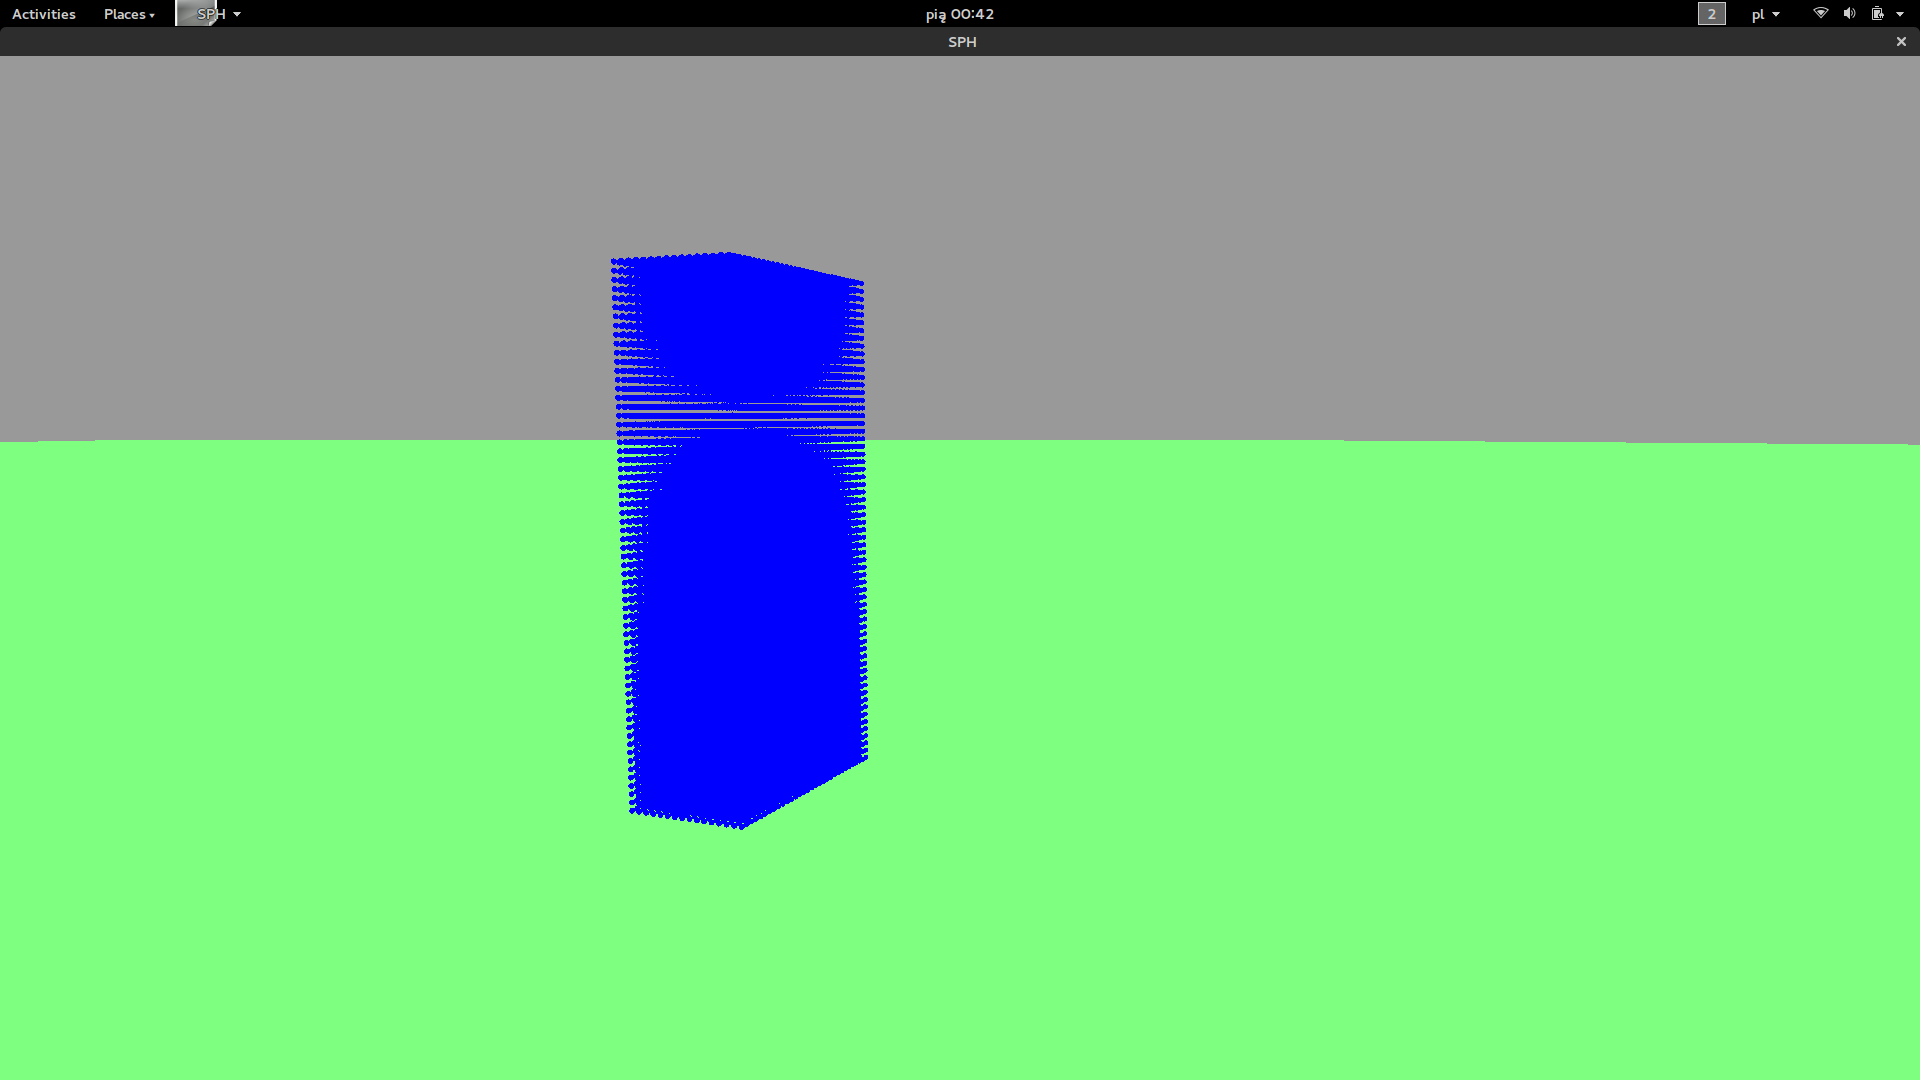
\includegraphics[width=0.49\textwidth]{1.png}
		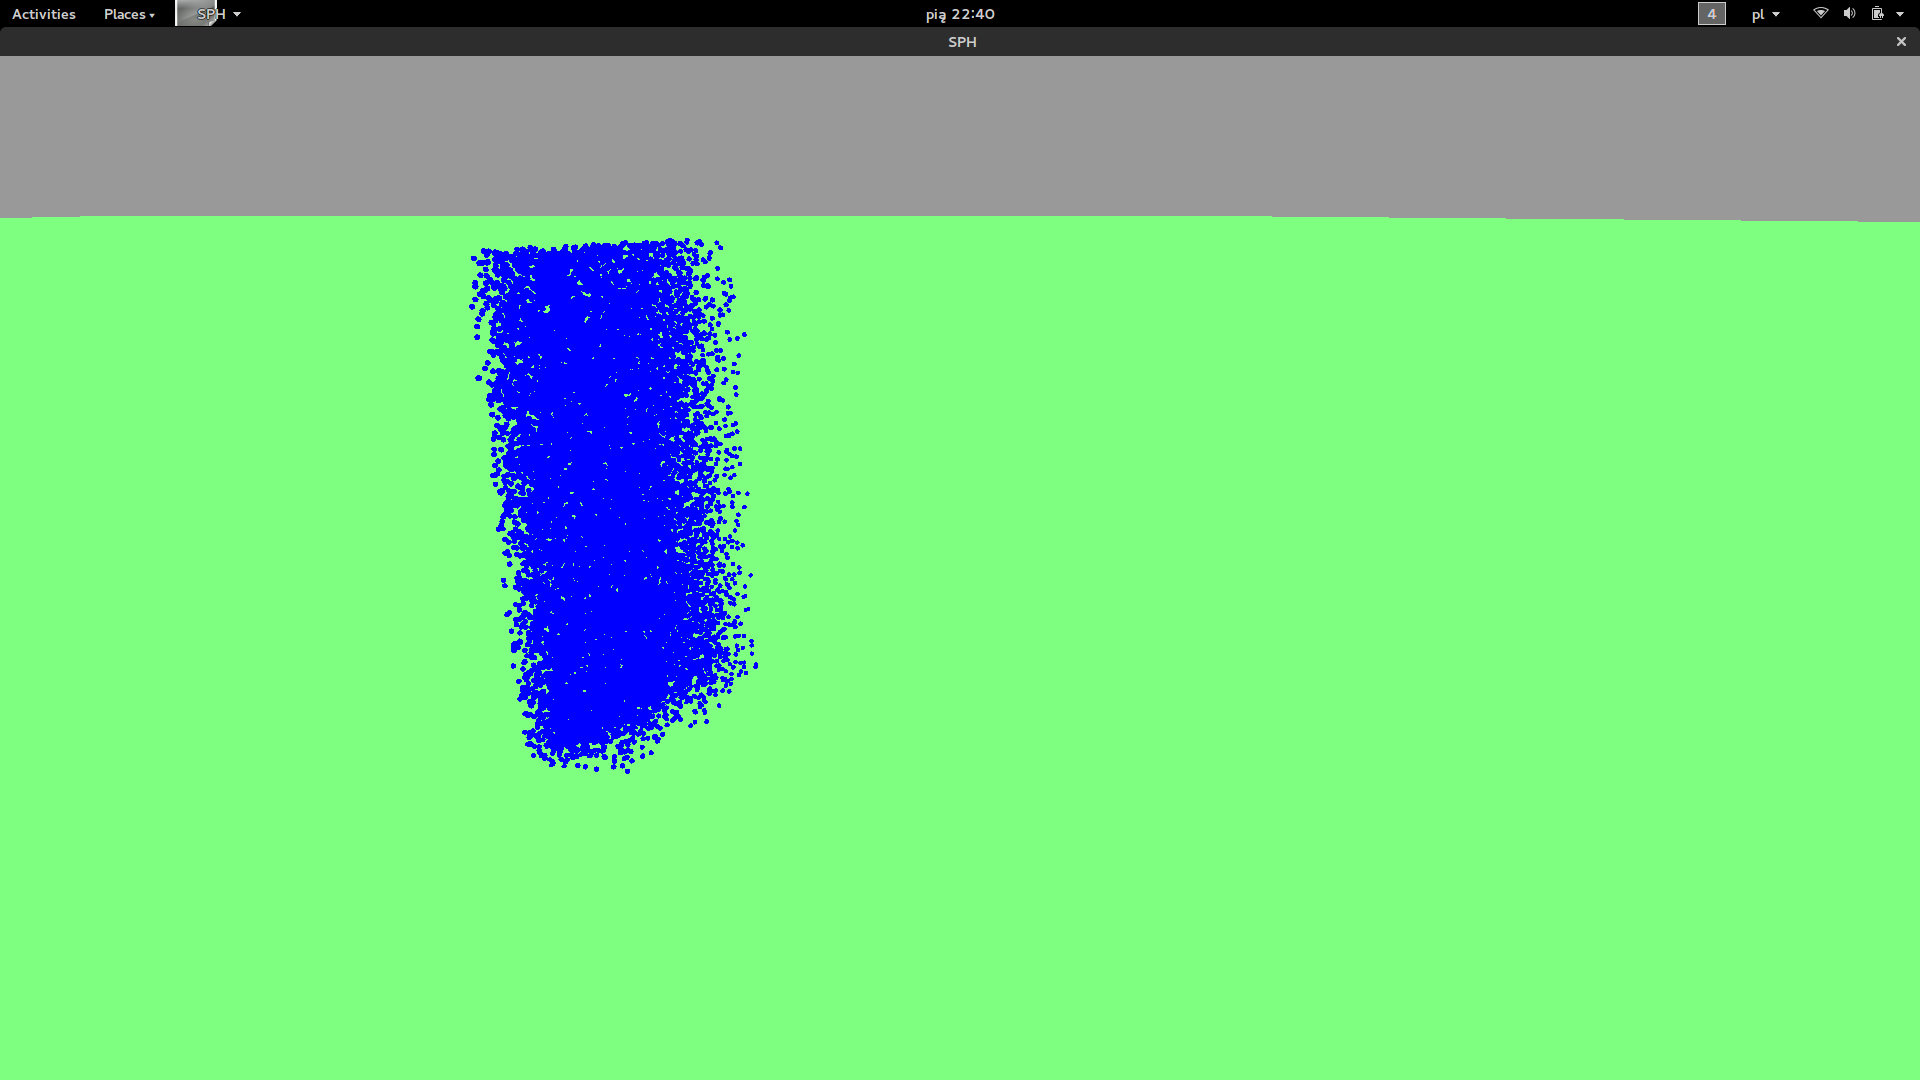
\includegraphics[width=0.49\textwidth]{2.png}
		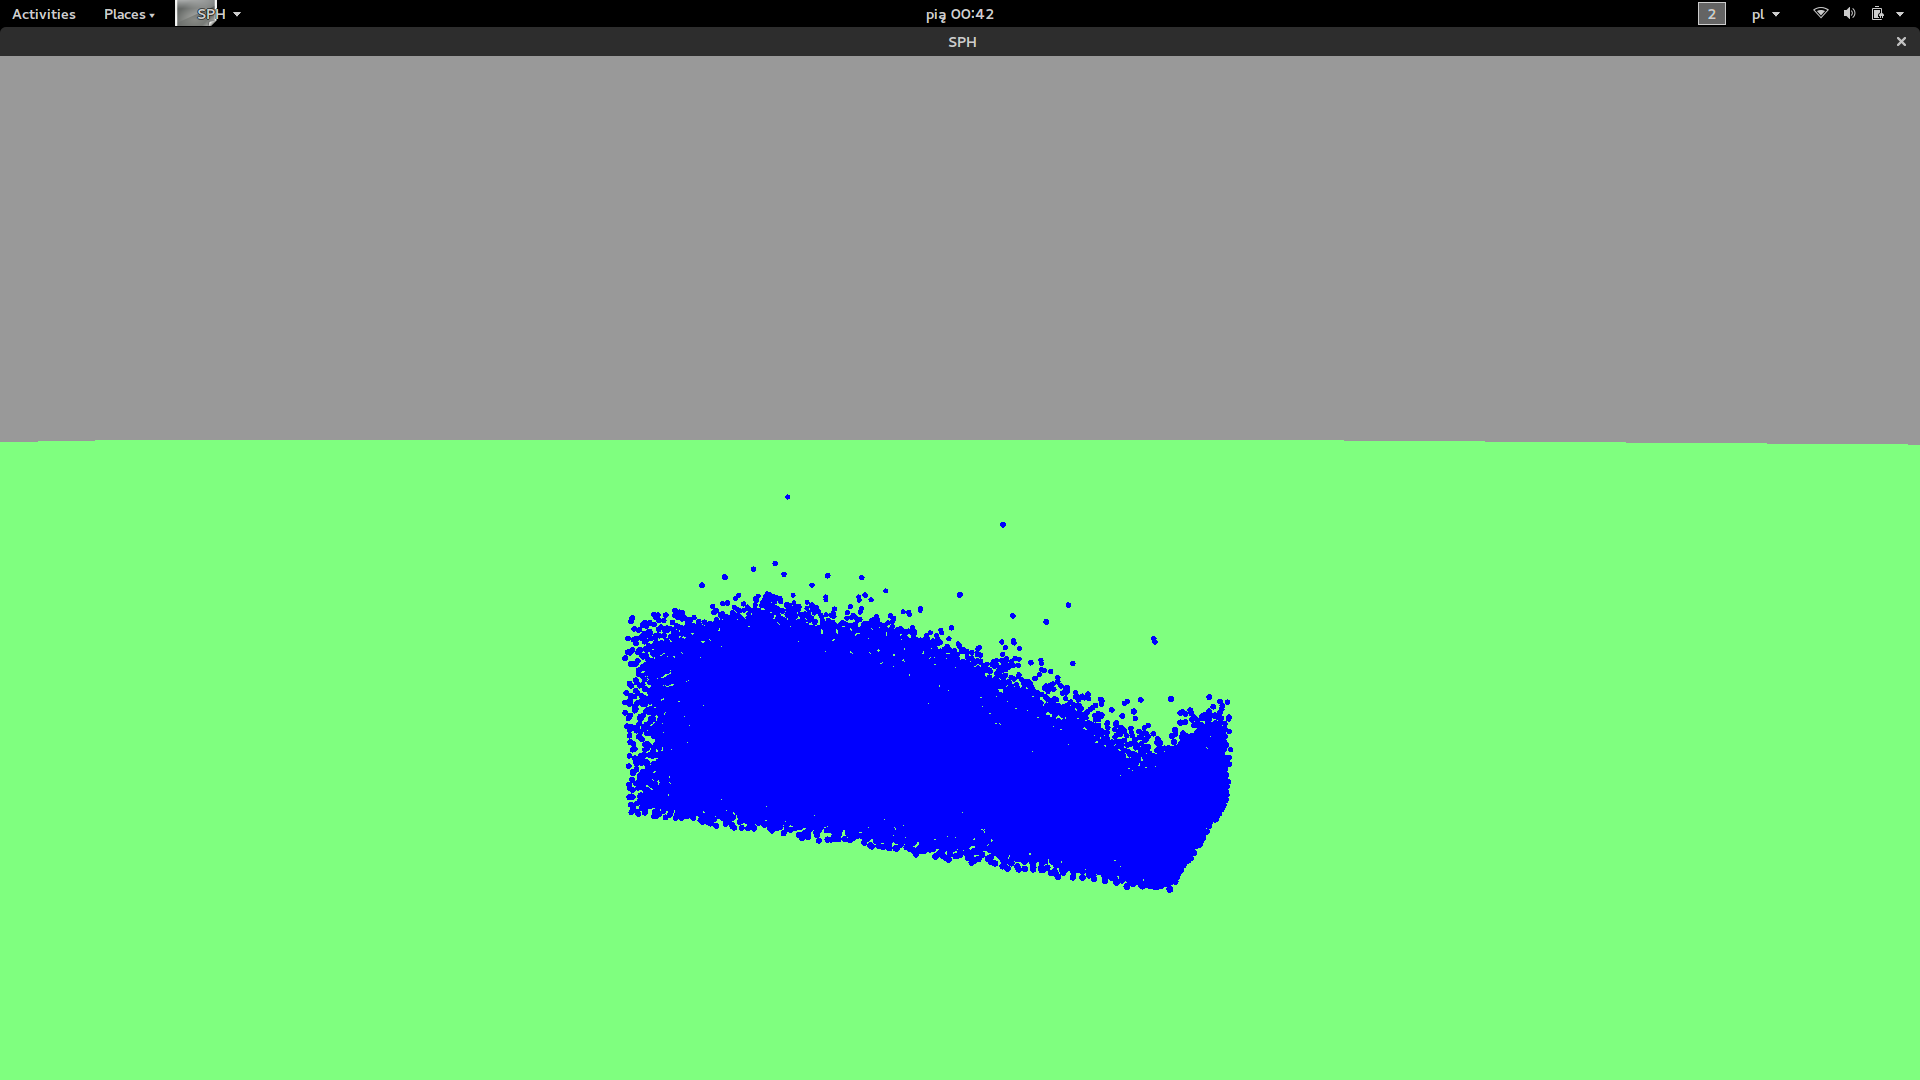
\includegraphics[width=0.49\textwidth]{3.png}
		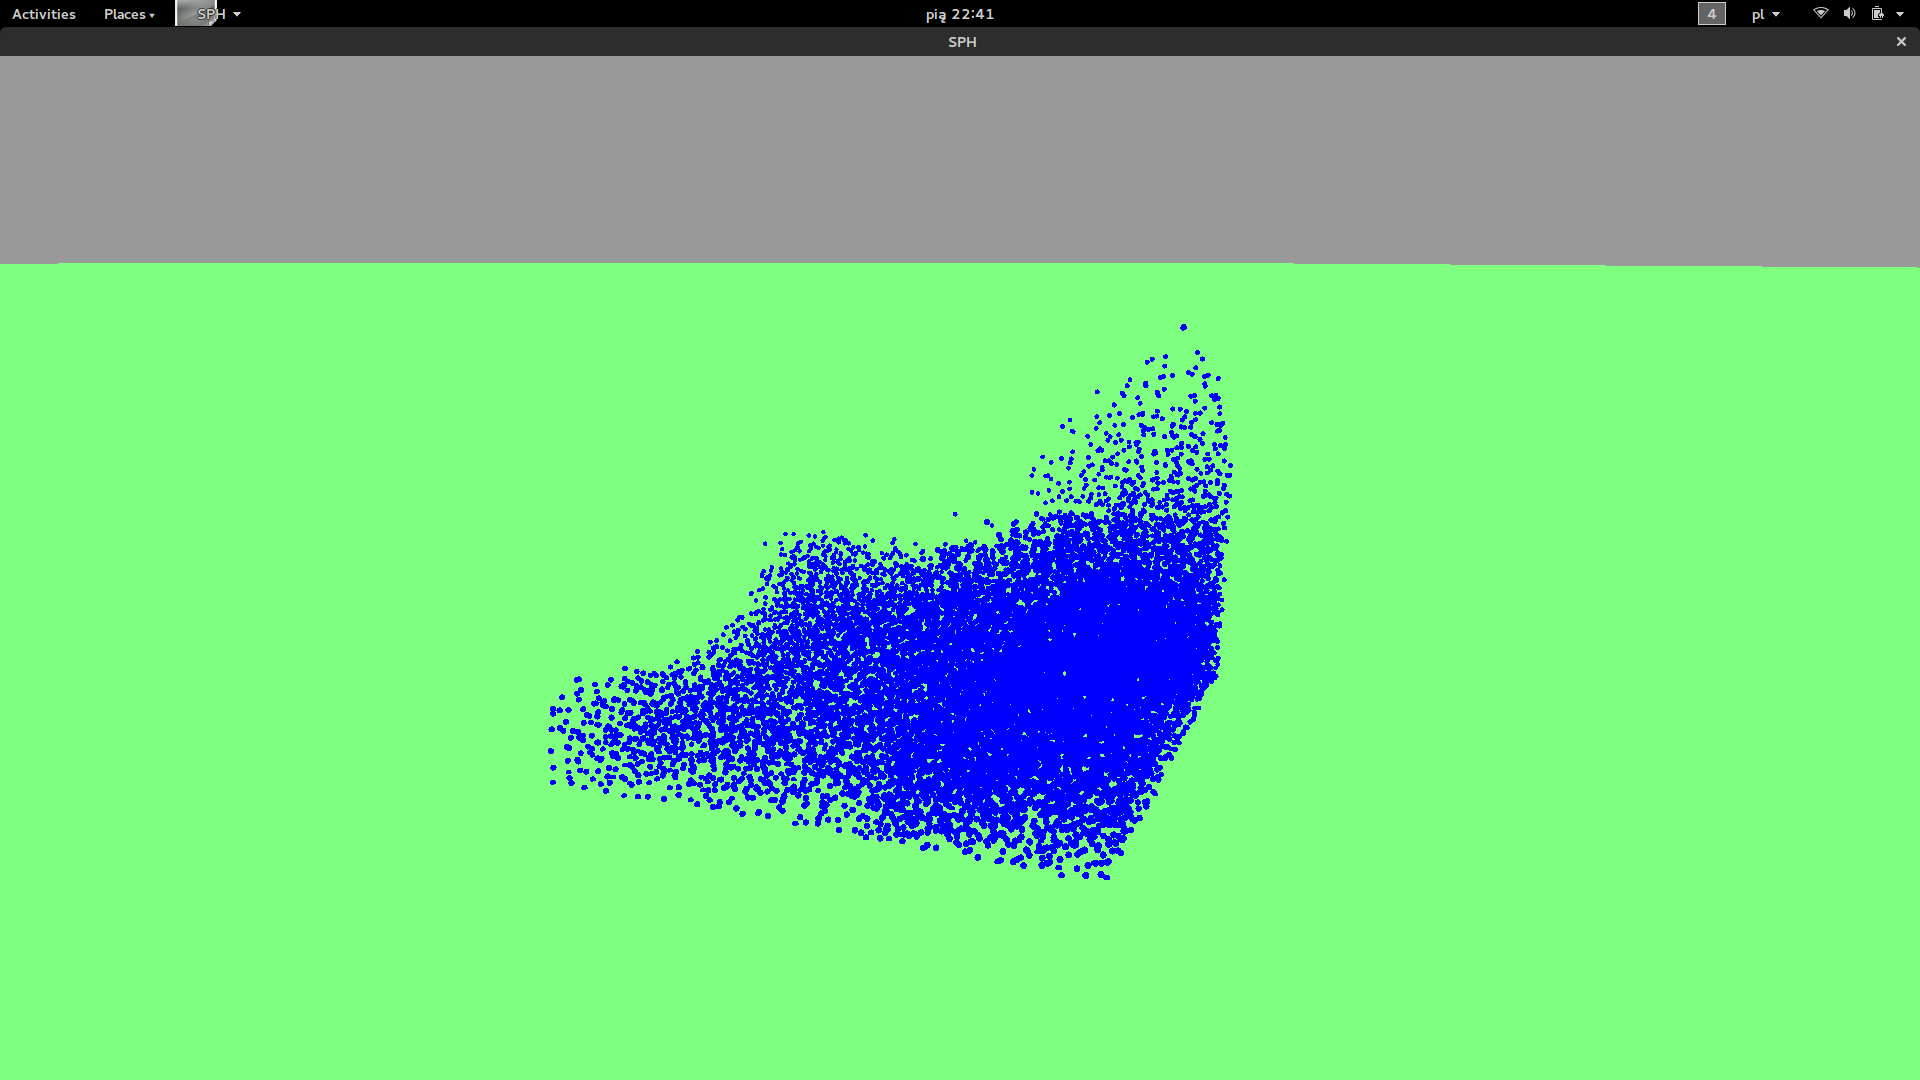
\includegraphics[width=0.49\textwidth]{4.png}
		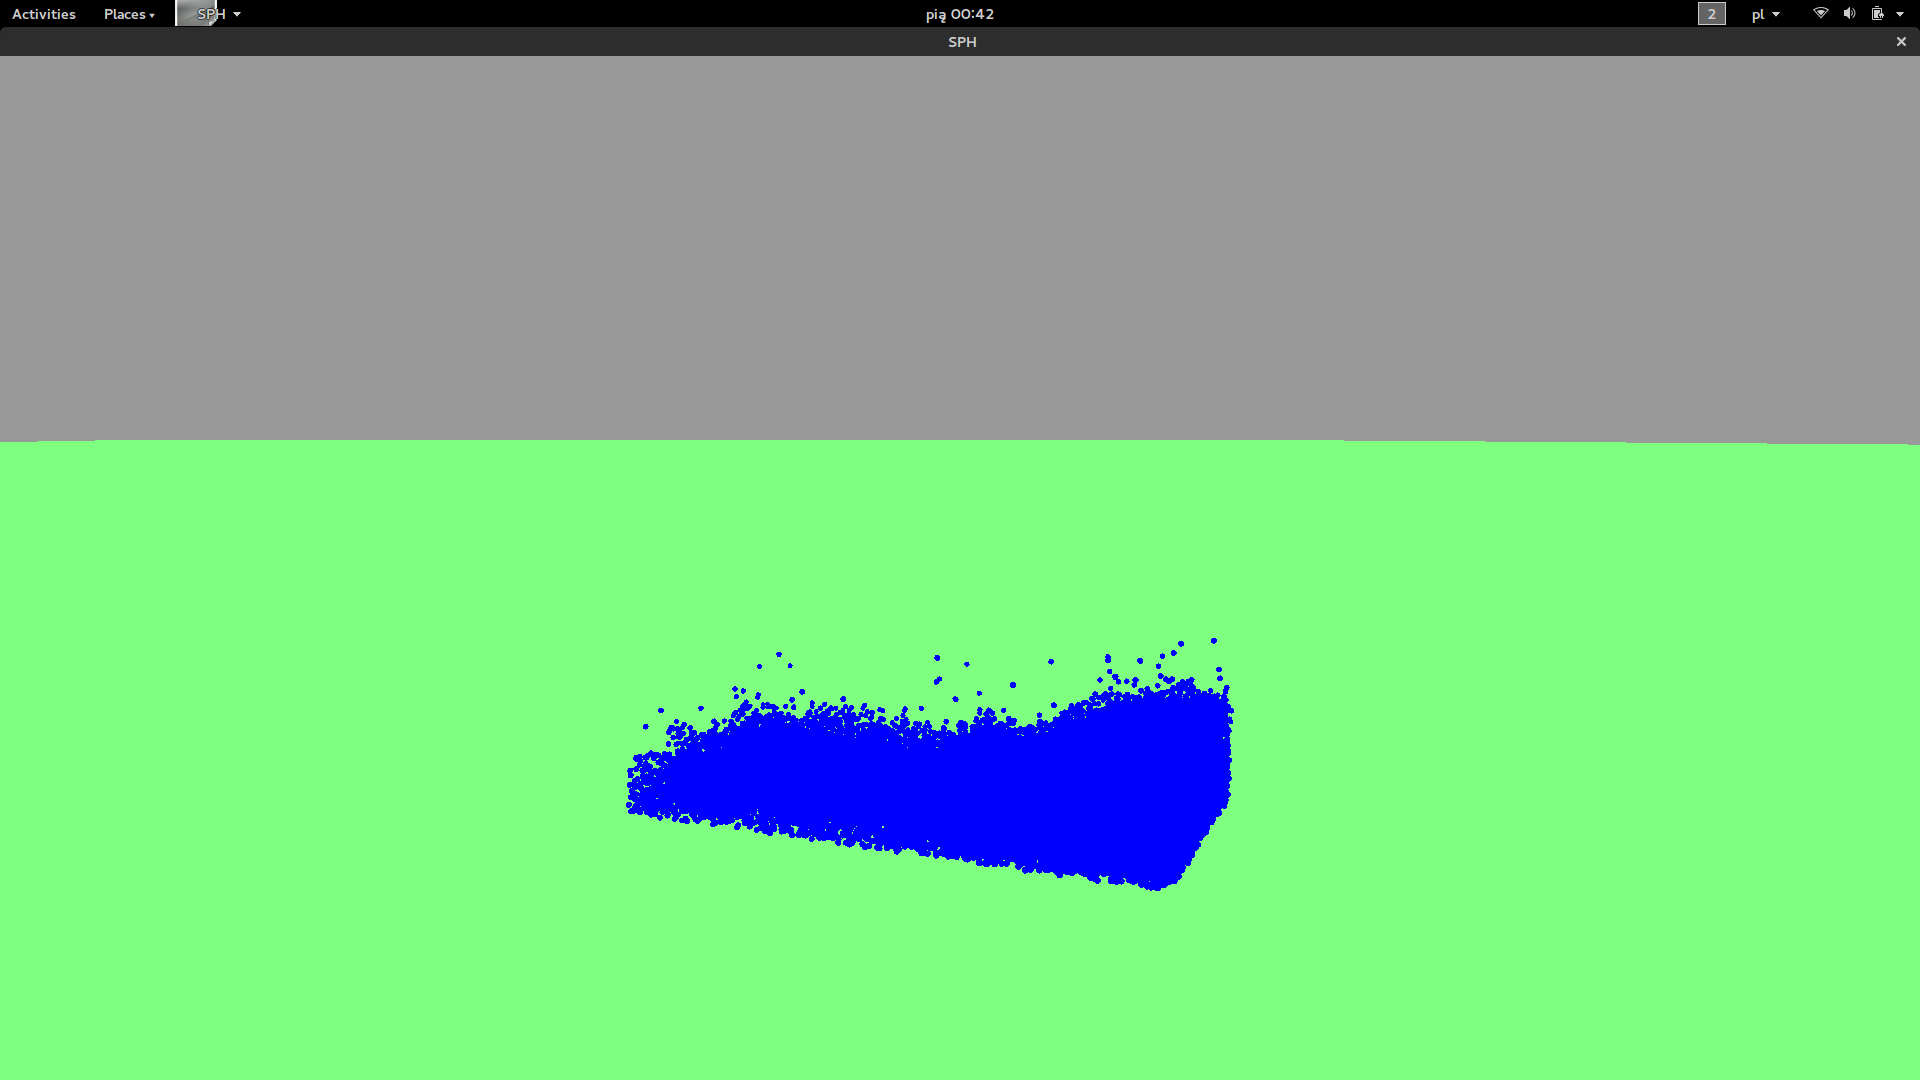
\includegraphics[width=0.49\textwidth]{5.png}
		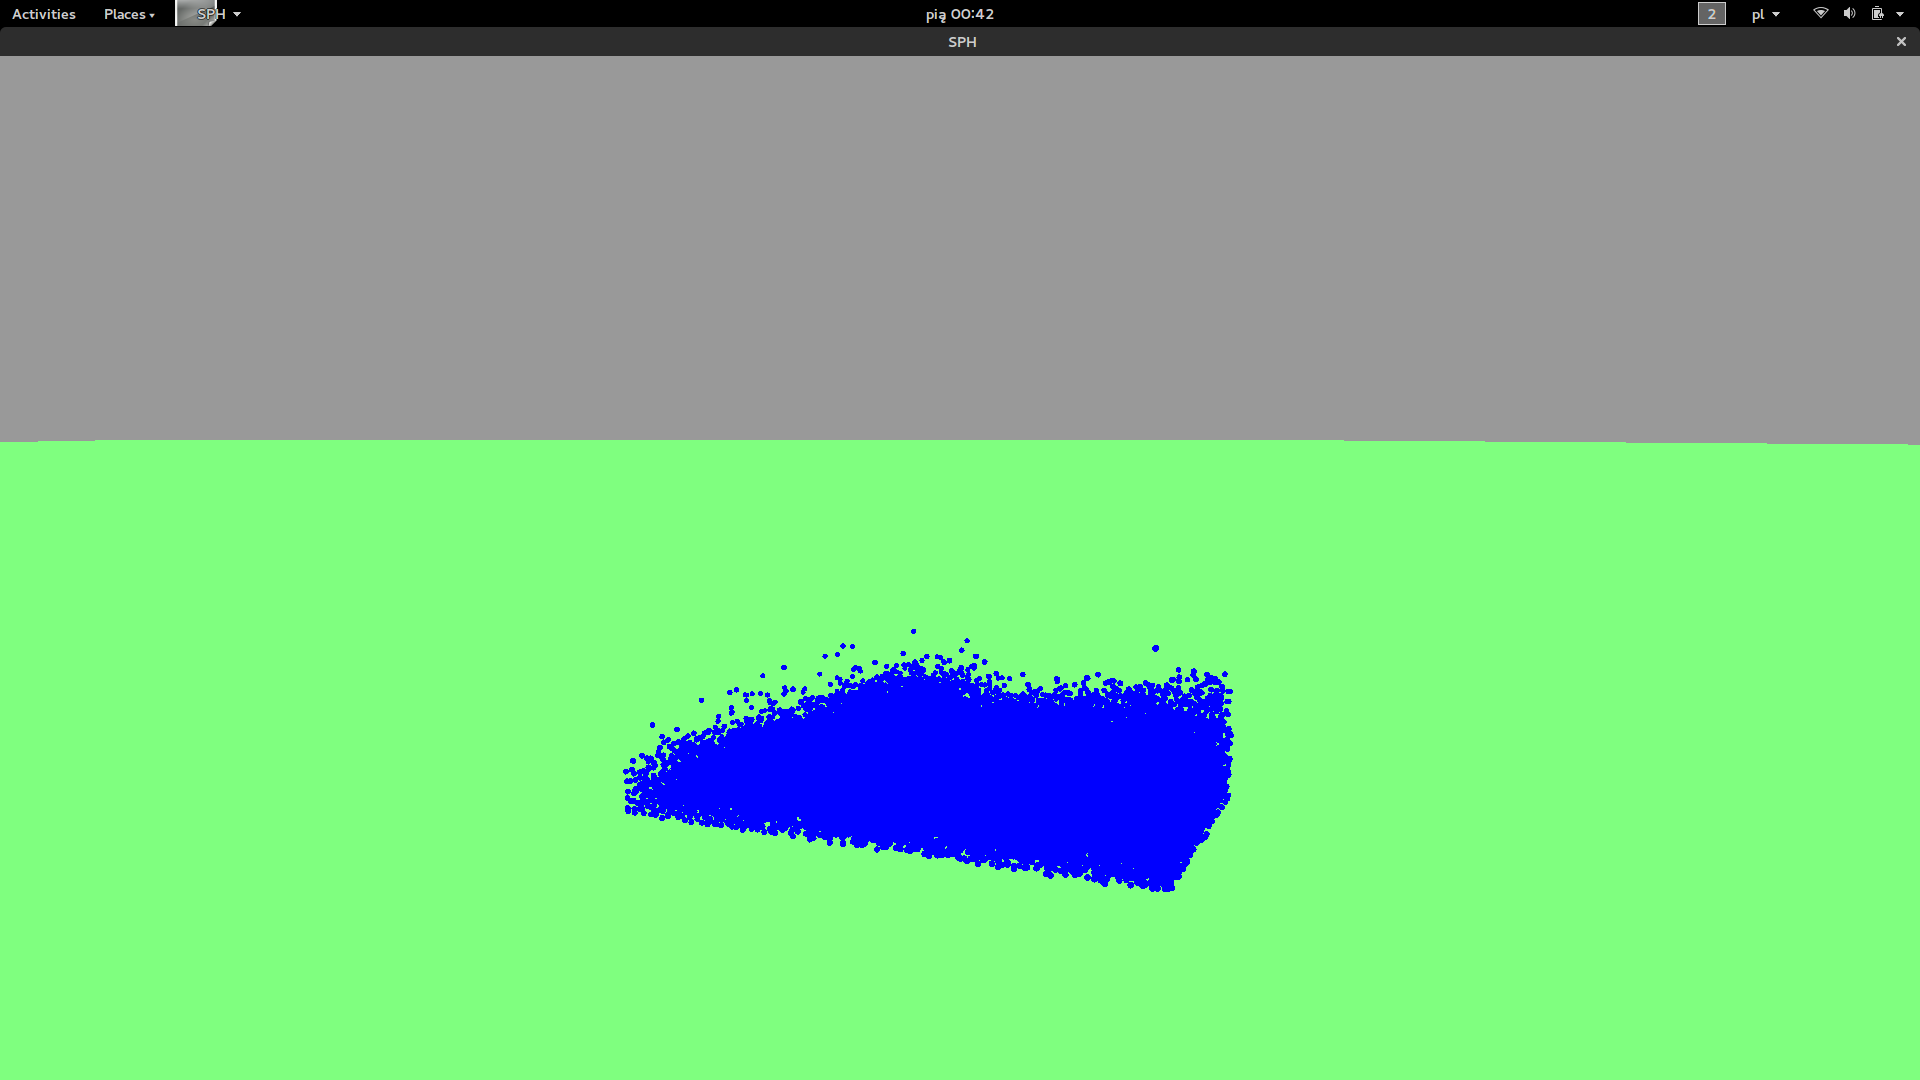
\includegraphics[width=0.49\textwidth]{6.png}
		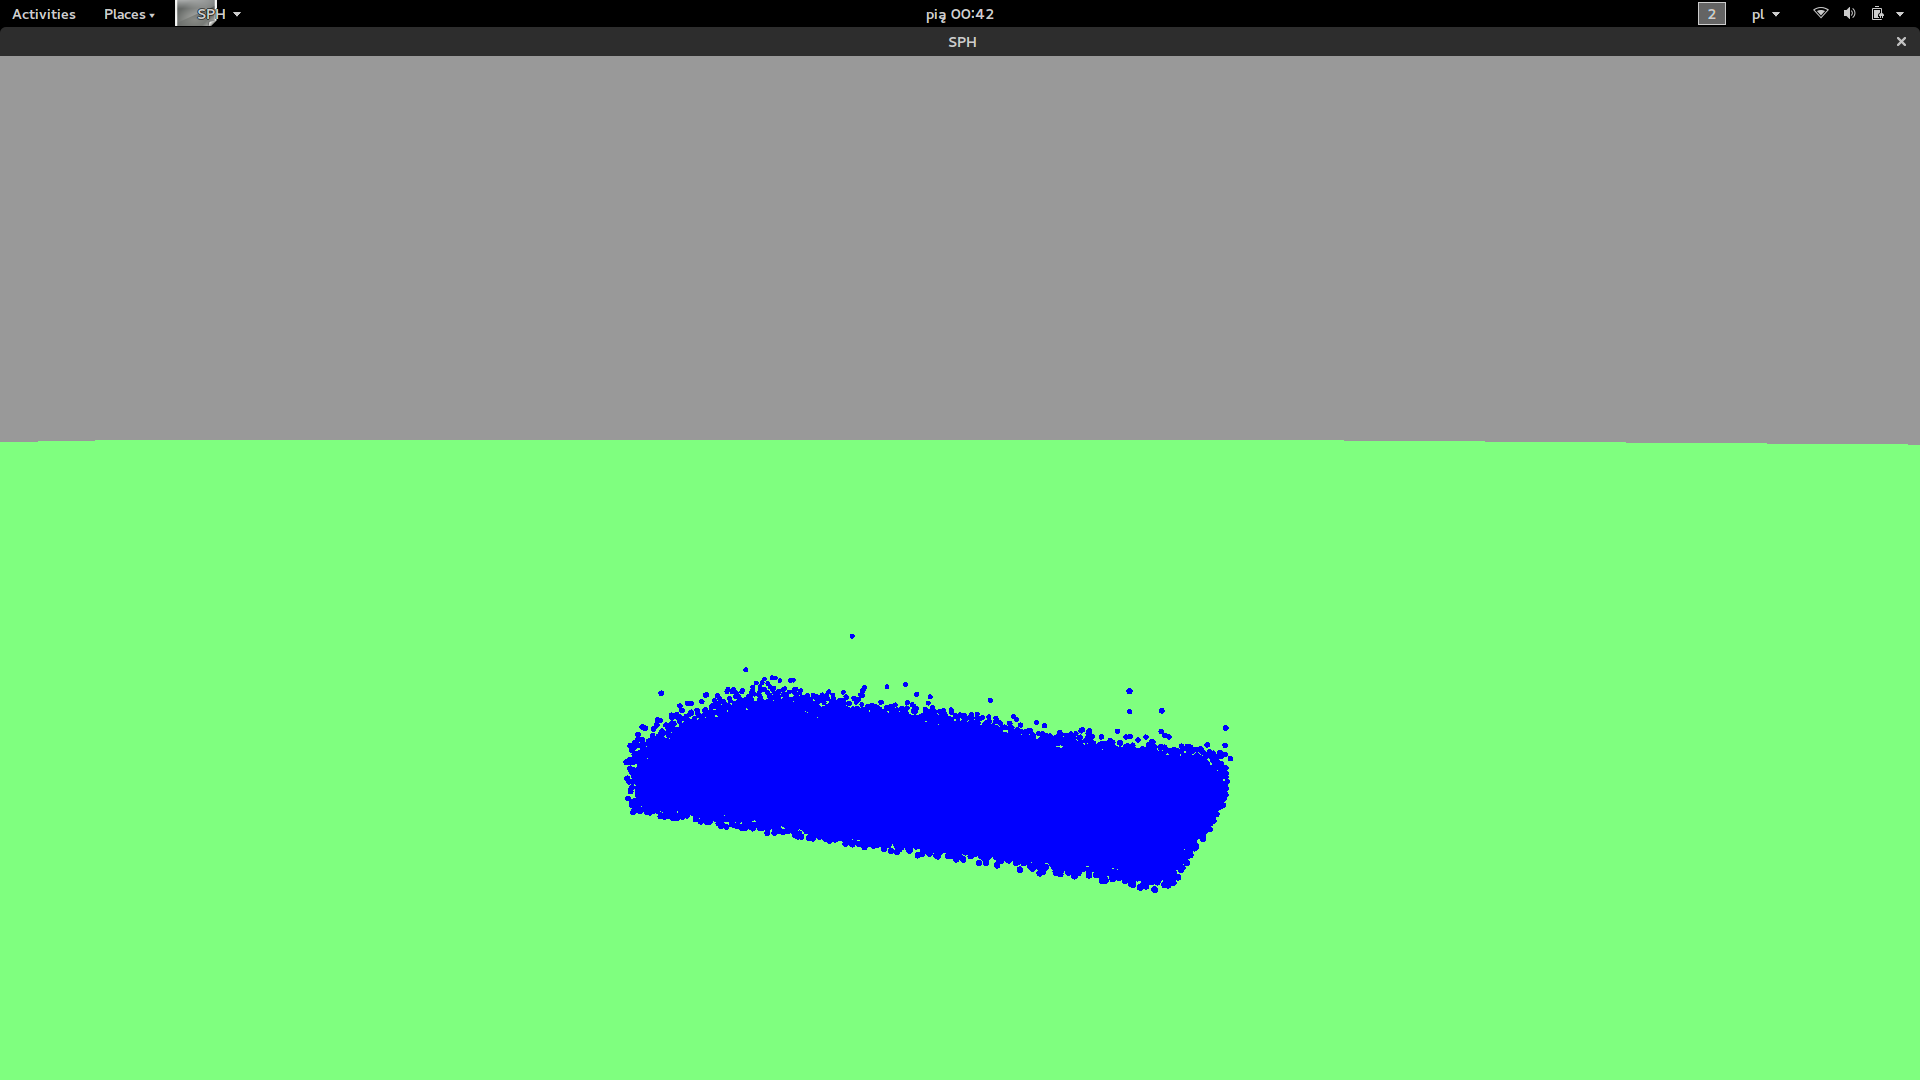
\includegraphics[width=0.49\textwidth]{7.png}
		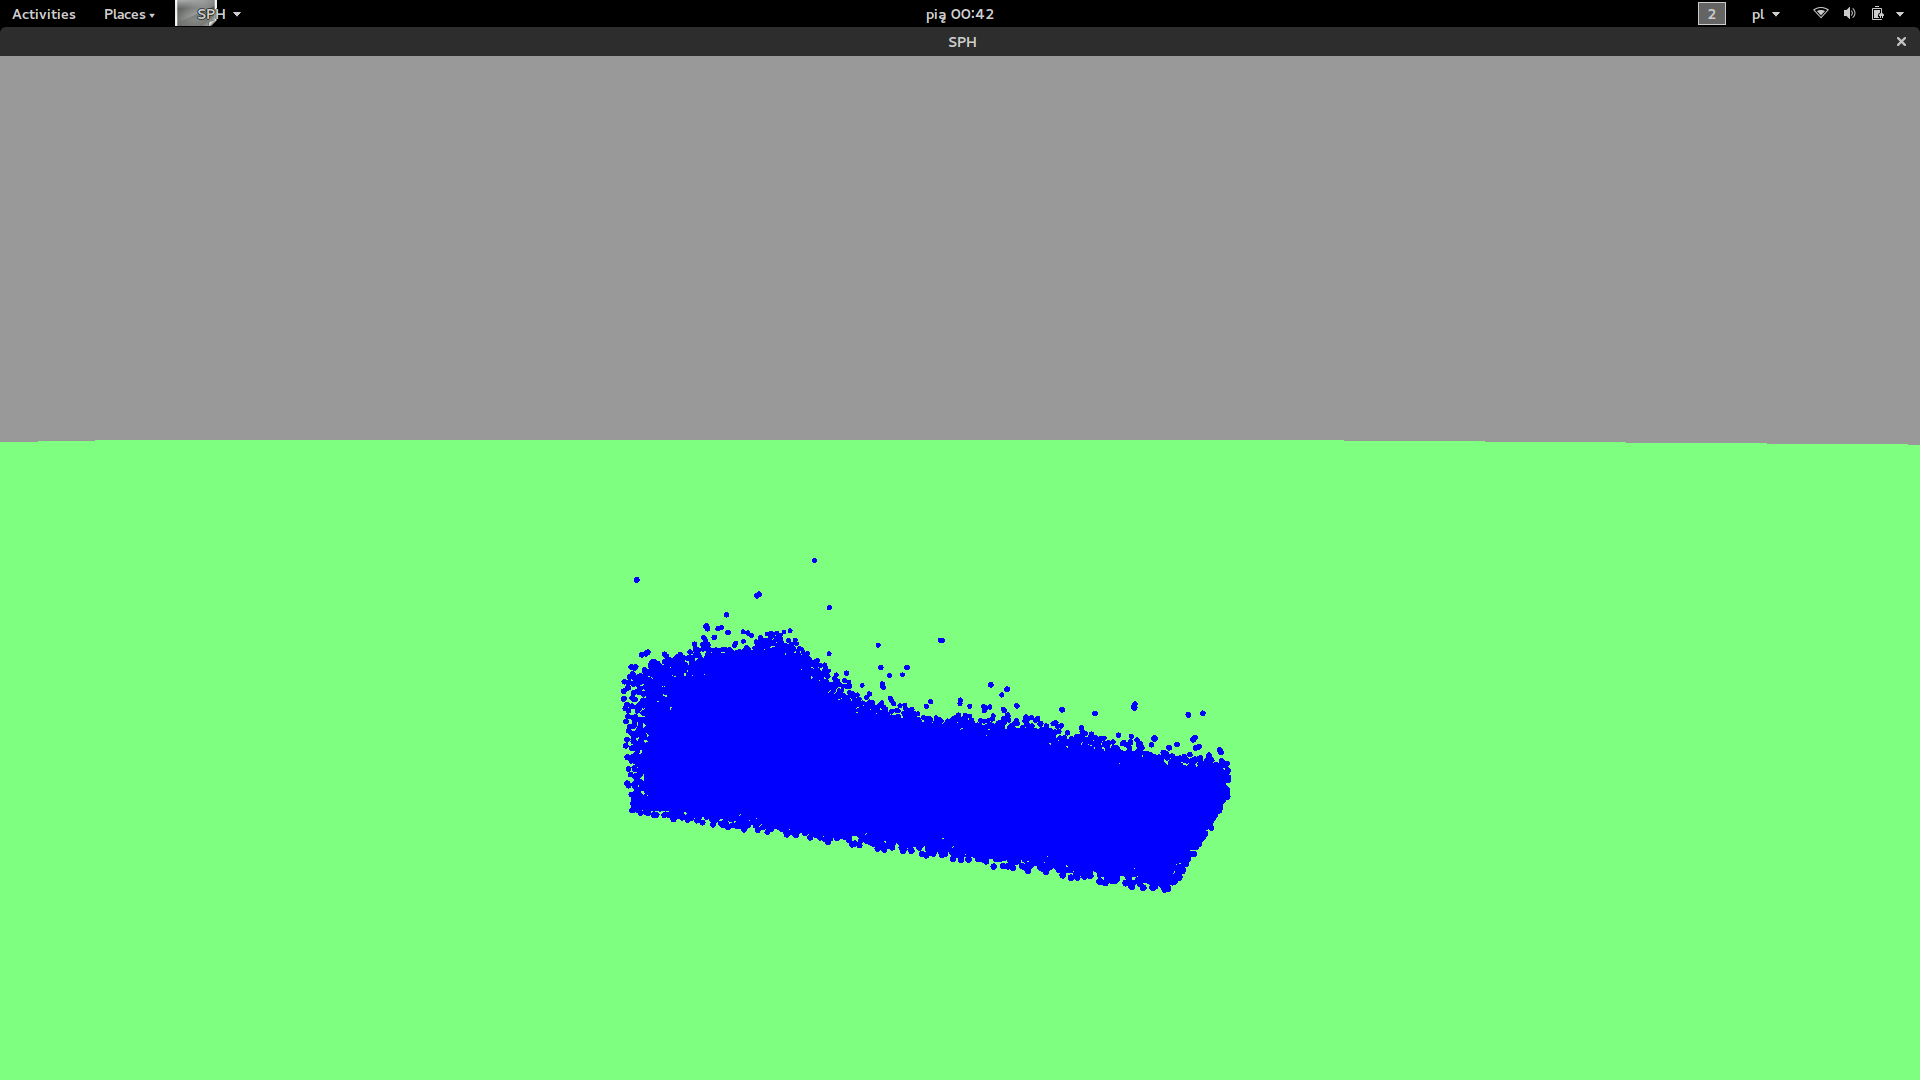
\includegraphics[width=0.49\textwidth]{8.png}
		\caption{Screenshoty z działania aplikacji}
	\end{figure}
			 
			 
	\nocite{OpenCLProgrammingGuide, SPHWebinar}

	\bibliography{bibliografia}
		
		
		
	
\end{document}
